%%%%%%%%%%%%%%%%%%%%%%%%%%%%%%%%%%%%%%%%%
% a0poster Landscape Poster
% LaTeX Template
% Version 1.0 (22/06/13)
%
% The a0poster class was created by:
% Gerlinde Kettl and Matthias Weiser (tex@kettl.de)
%
% This template has been downloaded from:
% http://www.LaTeXTemplates.com
%
% License:
% CC BY-NC-SA 3.0 (http://creativecommons.org/licenses/by-nc-sa/3.0/)
%
%%%%%%%%%%%%%%%%%%%%%%%%%%%%%%%%%%%%%%%%%

%-------------------------------------------------------------------------------
%	PACKAGES AND OTHER DOCUMENT CONFIGURATIONS
%-------------------------------------------------------------------------------

\documentclass[a0, landscape]{a0poster}

\usepackage{multicol} % This is so we can have multiple columns of text side-by-side
\columnsep=100pt % This is the amount of white space between the columns in the poster
\columnseprule=3pt % This is the thickness of the black line between the columns in the poster

\usepackage[svgnames]{xcolor} % Specify colors by their 'svgnames', for a full list of all colors available see here: http://www.latextemplates.com/svgnames-colors

%\usepackage{times} % Use the times font
\usepackage{palatino} % Uncomment to use the Palatino font
\usepackage{graphicx} % Required for including images
\graphicspath{{figures/}} % Location of the graphics files
\usepackage{booktabs} % Top and bottom rules for table
\usepackage[font=small,labelfont=bf]{caption} % Required for specifying captions to tables and figures
\usepackage{amsfonts, amsmath, amsthm, amssymb} % For math fonts, symbols and environments
\usepackage{wrapfig} % Allows wrapping text around tables and figures

\begin{document}

%----------------------------------------------------------------------------------------
%	POSTER HEADER
%----------------------------------------------------------------------------------------

% The header is divided into three boxes:
% The first is 55% wide and houses the title, subtitle, names and university/organization
% The second is 25% wide and houses contact information
% The third is 19% wide and houses a logo for your university/organization or a photo of you
% The widths of these boxes can be easily edited to accommodate your content as you see fit

\begin{minipage}[b]{0.85\linewidth}
\veryHuge \color{NavyBlue} \textbf{Evaluating the accuracy of diffusion MRI models in the Human Connectome Project at scale with DIPY and Cloudknot} \color{Black}\\ % Title
%\Huge\textit{An Exploration of Complexity}\\[1cm] % Subtitle
\huge \textbf{Ariel Rokem\textsuperscript{1}, \& Adam Richie-Halford \textsuperscript{2}}\\ % Author(s)
\Large 1. The eScience Institute, 2. Dept. of Physics, Univ. of Washington \\ % University/organization
\Large Contact: \texttt{arokem@uw.edu} $|$ Download: \texttt{http://arokem.org/presentations/brainpi-dipy-2019}
\end{minipage}
%
%\begin{minipage}[b]{0.25\linewidth}
%\color{DarkSlateGray}\Large \textbf{Contact Information:}\\
%Department Name\\ % Address
%University Name\\
%123 Broadway, State, Country\\\\
%Phone: +1 (000) 111 1111\\ % Phone number
%Email: \texttt{john@LaTeXTemplates.com}\\ % Email address
%\end{minipage}
%
\begin{minipage}[b]{0.19\linewidth}

\includegraphics[width=10cm]{UWlogo.png}
\end{minipage}

\vspace{0.5cm} % A bit of extra whitespace between the header and poster content

%----------------------------------------------------------------------------------------

\begin{multicols}{3} % This is how many columns your poster will be broken into, a poster with many figures may benefit from less columns whereas a text-heavy poster benefits from more

%----------------------------------------------------------------------------%	Introduction
%----------------------------------------------------------------------------

\section*{Introduction}

\subsection*{The Human Connectome Project}

Diffusion MRI (dMRI) measurements provide detailed information about human brain
connectivity and microstructure \emph{in vivo}. HCP has measured high-quality
multi-modal MRI data from 1,200 individuals and is making these data publcly
available \cite{glasser2016}. Data can be accessed through Amazon's Simple
Storage Web Service (S3).

\subsection*{What model should we use to explain the data?}

\subsection*{Diffusion Tensor Imaging (DTI): 6 parameters}

Approximates diffusion in every voxel as a Gaussian distribution
\cite{Basser1994-hg}:

\vspace{2mm}
\begin{center}
\begin{large}

$S(\theta, b) = S_0 e^{\theta^T \mathbf{Q} \theta} $

\end{large}
\end{center}

\noindent $b$ is the \textbf {b-value},

\noindent $S_0$ is the signal in the absence of diffusion gradient sensitization ($b=0$)

\noindent $\mathbf{Q}$ is a positive-definite quadratic form:

\vspace{2mm}
\begin{center}

$\mathbf{D} = \begin{pmatrix} \sigma_{xx} & \sigma_{xy} & \sigma_{xz} \\
                              \sigma_{yx} & \sigma_{yy} & \sigma_{yz} \\
				                      \sigma_{zx} & \sigma_{zy} & \sigma_{zz} \\
\end{pmatrix} $

\end{center}

\subsection*{Diffusion Kurtosis imaging (DKI): 21 parameters}

DKI is an extension of DTI that accounts for non-Gaussian behavior in complex tissue, with many barriers to the diffusion process (cell membranes,
myelin sheaths, etc.) \cite{Jensen2005-vr}:

\vspace{2mm}
\begin{center}
\begin{large}

$ S(\theta, b)=S_{0}e^{-bD(\theta)+\frac{1}{6}b^{2}D(\theta)^{2}K(\theta)}$

\vspace{2mm}
\end{large}
\end{center}

\vspace{2mm}
\begin{center}
\begin{large}

$D(\theta)=\sum_{i=1}^{3}\sum_{j=1}^{3}\theta_{i}\theta_{j}Q_{ij}$

\vspace{2mm}
\end{large}
\end{center}

\vspace{2mm}
\begin{center}
\begin{large}

$K(\theta)=\frac{MD^{2}}{D(\theta)^{2}}\sum_{i=1}^{3}\sum_{j=1}^{3}\sum_{k=1}^{3} \sum_{l=1}^{3}\theta_{i}\theta_{j}\theta_{k}\theta_{l}W_{ijkl}$

\vspace{2mm}
\end{large}
\end{center}

$\mathbf{W}$ is a rank 4 tensor (3-by-3-by-3-by-3 matrix).

\vspace{-2mm}
\subsection*{Diffusion Statistics}

\begin{itemize}

\item Mean diffusivity (\textbf{MD}) characterizes the mean displacement of
water molecules within a voxel.

\item Fractional anisotropy (\textbf{FA}) characterizes the variance in
diffusivity in different directions.

\end{itemize}

\large

\noindent \textbf{Brain measurements that provide a close tie between brain tissue properties and behavior}.

\vfill
\columnbreak

\color{Navy}
%----------------------------------------------------------------------------%	RESULTS
%----------------------------------------------------------------------------

\section*{Cloud computing}

Cloud computing provides access to data and compute resources in a manner that is:

\begin{itemize}
\item{{\bf Scalable}. Massive compute resources can be deployed.}
\item{{\bf Elastic}. Resources can be provisioned and de-provisioned rapidly.}
\item{{\bf Robust}. Can handle large datasets and workloads.}
\item{{\bf Up to date}. The underlying compute technologies are updated by the cloud provider.}
\end{itemize}

But it is also:

\begin{itemize}
\item{{\bf Challenging to learn.} Researchers using the cloud need to learn new terminology.}
\item{{\bf Hard to automate.} Complex APIs vs. clicking through web consoles.}
\item{{\bf Provisioning resources has overhead.} Especially in the absence of automation.}
\item{{\bf Not (yet?) a perfect match to scientific use-cases.} The major business case is developers building web-based platforms.}
\end{itemize}

\subsection*{Cloudknot}

A Python library that automates submission of scientific computing functions
to the Amazon Web Services Batch service.

\texttt{https://richford.github.io/cloudknot/}

\section*{Results}

\noindent \textbf{We compared DKI and DTI using \emph{K-fold cross-validation}}

\noindent \textbf{We estimated model fit \emph{accuracy} and model parameter \emph{reliability}}

\subsection*{Model accuracy}
\normalsize

\noindent Cross-validated $R^2$: \textbf{A} Comparison of the full distribution
in a single subject, and comparison of the median (dashed line) in all subjects
for DKI (all b-values) and DTI (\textbf{B} all b-values, \textbf{C} only b=1,000
$s/mm^2$  \hfill \break

\begin{minipage}[b]{1\linewidth}
  \large
  \begin{minipage}[b]{0.33\linewidth}
  \textbf{A}\\
  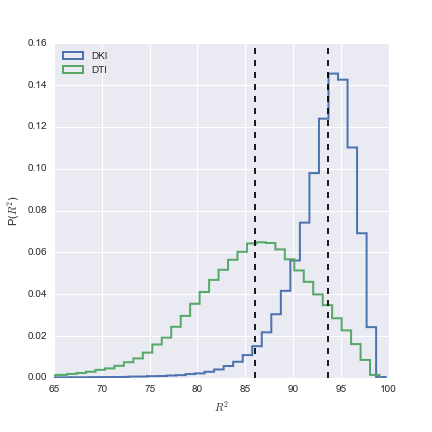
\includegraphics[width=11.5cm]{histogram_cod_dki_dti.png}
  \end{minipage}
  \begin{minipage}[b]{0.33\linewidth}
  \textbf{B}\\
  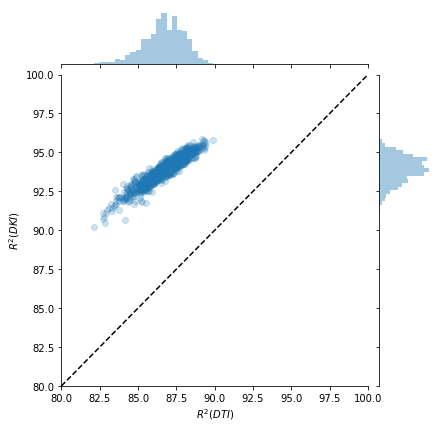
\includegraphics[width=11.5cm]{cod_dti_dki.png}
  \end{minipage}
  \begin{minipage}[b]{0.33\linewidth}
  \textbf{C}\\
  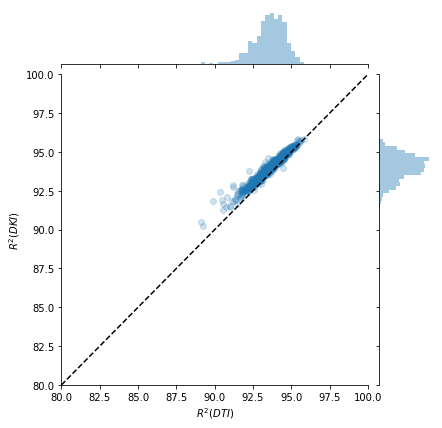
\includegraphics[width=11.5cm]{dti_1000_dki.png}
  \end{minipage}
\end{minipage}

\subsection*{Parameter reliability}

\noindent Parameter reliability is estimated by comparing diffusion-based
statistics based on a difference in FA/MD between b=1000 and b=1000,2000 (DTI)
or between b=1000,2000, b=1000,3000 (DKI).

\noindent BIAS is the median difference between sub-samples VARIABILITY is the
range of the differences (the range of the central 95\% of the distribution).

\subsubsection*{Mean diffusivity}

\begin{minipage}[b]{1\linewidth}
  \begin{minipage}[b]{0.33\linewidth}
  \center Single subject distributions\\
  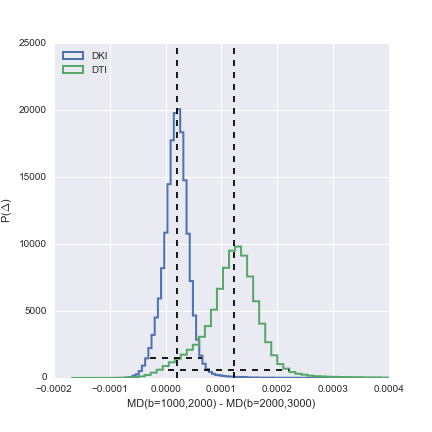
\includegraphics[width=11.5cm]{reliability_singleton_md.png}
  \end{minipage}
  \begin{minipage}[b]{0.33\linewidth}
    \center Bias\\
    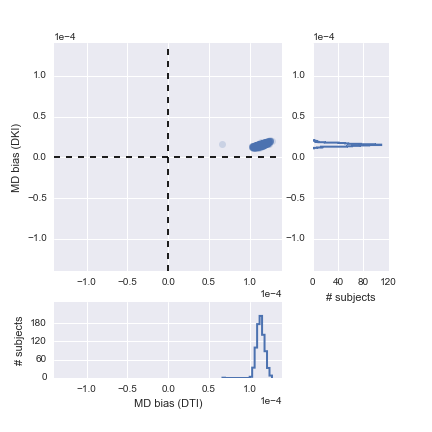
\includegraphics[width=11.5cm]{md_bias.png}
  \end{minipage}
  \begin{minipage}[b]{0.33\linewidth}
    \center Variability\\
  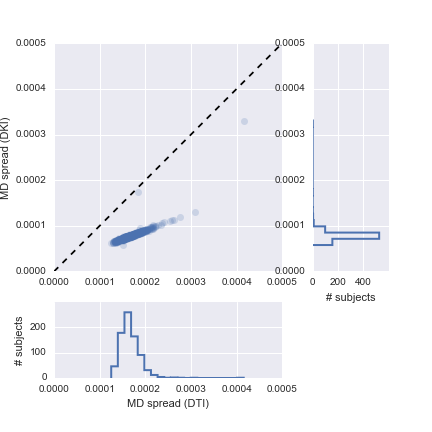
\includegraphics[width=11.5cm]{md_spread.png}
  \end{minipage}
\end{minipage}

\subsubsection*{Fractional anisotropy}

\begin{minipage}[b]{1\linewidth}
  \begin{minipage}[b]{0.33\linewidth}
  \center Single subject distributions\\
  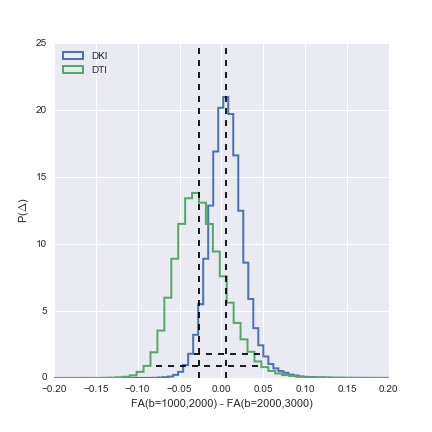
\includegraphics[width=11.5cm]{reliability_singleton_fa.png}
  \end{minipage}
  \begin{minipage}[b]{0.33\linewidth}
    \center Bias\\
    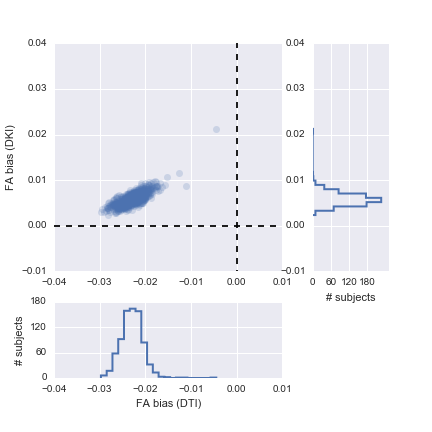
\includegraphics[width=11.5cm]{fa_bias.png}
  \end{minipage}
  \begin{minipage}[b]{0.33\linewidth}
    \center Variability\\
  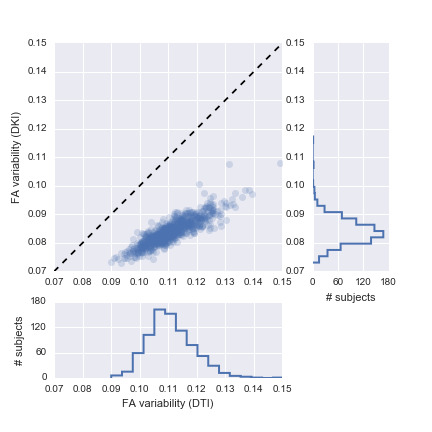
\includegraphics[width=11.5cm]{fa_spread.png}
  \end{minipage}
\end{minipage}

%----------------------------------------------------------------------------
%	MATERIALS AND METHODS
%----------------------------------------------------------------------------
\normalsize
\section*{Materials and Methods}
\vspace{-10mm}
\subsection*{Data}
Measurements were obtained from the WU-Minn Human Connectome Project consortium
(\texttt{https://www.humanconnectome.org/}) through AWS S3.

\noindent Of the 900 subjects that are available, 788 subjects have full
diffusion measurements: 270 diffusion weighted directions in 3 different
b-values (90 directions each): 1,000, 2,000 and 3,000 $s/mm^2$, collected at
1.25 x 1.25 x 1.25 $mm^3$ resolution.

\noindent \emph{Freesurfer} segmentation from a T1-weighted measurement was also
used. We focused our analysis only on the parts of the volume that contained the
white matter. \vspace{-10mm}


\color{DarkSlateGray}
\subsection*{Analysis}

We used an Amazon Web Services compute cluster with 36 nodes. AWS
\emph{r3.2xlarge} instances were used, optimized for memory-intensive
applications: each instance has 8 vCPU, 61 GiB Memory and 160 GB SSD storage.

\noindent We used DTI and DKI implementations that are part of the DIPY
open-source software library (\texttt{http://dipy.org/}) \cite{Garyfallidis2014FrontNeuroinf}. 5-fold cross-validation was implemented using DIPY's cross-validation module \cite{Rokem2015PLoS}

\noindent Computation was distributed using Apache Spark, an open-source
parallel processing framework that coordinates computation across distributed
clusters (\texttt{http://spark.apache.org/}). Because model-fitting requires
large amounts of memory, each compute node ran one Spark worker.

\hspace{2 mm}

\includegraphics[height=3.5cm]{AWS.png}
\hspace{2 mm}

\includegraphics[height=3.5cm]{dipy-logo.png}
\hspace{2 mm}

\includegraphics[height=3.5cm]{spark-logo.png}
\hspace{2 mm}

\noindent Analysis software: \texttt{http://github.com/arokem/dki-accuracy-reliability}

%------------------------------------------------

\color{SaddleBrown} % SaddleBrown color for the conclusions to make them stand out

\section*{Conclusions}
\large
\begin{itemize}

\item DKI more accurately fits the HCP data than DTI

\item DKI statistics are more reliable than DTI statistics

\item DKI has the additional benefit that it provides additional parameters that
lend themselves to a richer biophysical interpretation of the signal.

\end{itemize}

\color{DarkSlateGray} % Set the color back to DarkSlateGray for the rest of the content

%---------------------------------------------------------------------------	REFERENCES
%----------------------------------------------------------------------------

\nocite{*} % Print all references regardless of whether they were cited in the poster or not
\bibliographystyle{plain} % Plain referencing style
\footnotesize \bibliography{poster} % Use the example bibliography file sample.bib

%----------------------------------------------------------------------------%	ACKNOWLEDGEMENTS
%----------------------------------------------------------------------------
\subsection*{Acknowledgements} \footnotesize This research was supported through
a grant from the Gordon \& Betty Moore Foundation and the Alfred P. Sloan
Foundation to the University of Washington eScience Institute, through NSF grant
IIS-1247469, and through gifts from Amazon and the Intel Science and Technology
Center for Big Data. We are also grateful for research cloud credits from Amazon
Web Services, and for a Google Summer of Code 2015 fellowship to RNH.


\includegraphics[height=2.6cm]{eSciencelogo.png}

\includegraphics[height=2.6cm]{SloanLogo.png}

\includegraphics[height=2.6cm]{MooreFdn.png}

\includegraphics[height=2.6cm]{NSFLogo}
%----------------------------------------------------------------------------

\end{multicols}
\end{document}
